\chapter{PCB
\index{Chapter!PCB}
\index{PCB}
\label{PCB}}
\section{Schematic}
\subsection{ORCad Capture Overview}
ORCad comes with a schematic software called Capture CIS which we used to create our schematics. As a reference to both us and others, this section is
dedicated to providing a small walkthrough to using the software and some nice-to-know features.
\begin{figure}[H]
  \scalebox{.3}{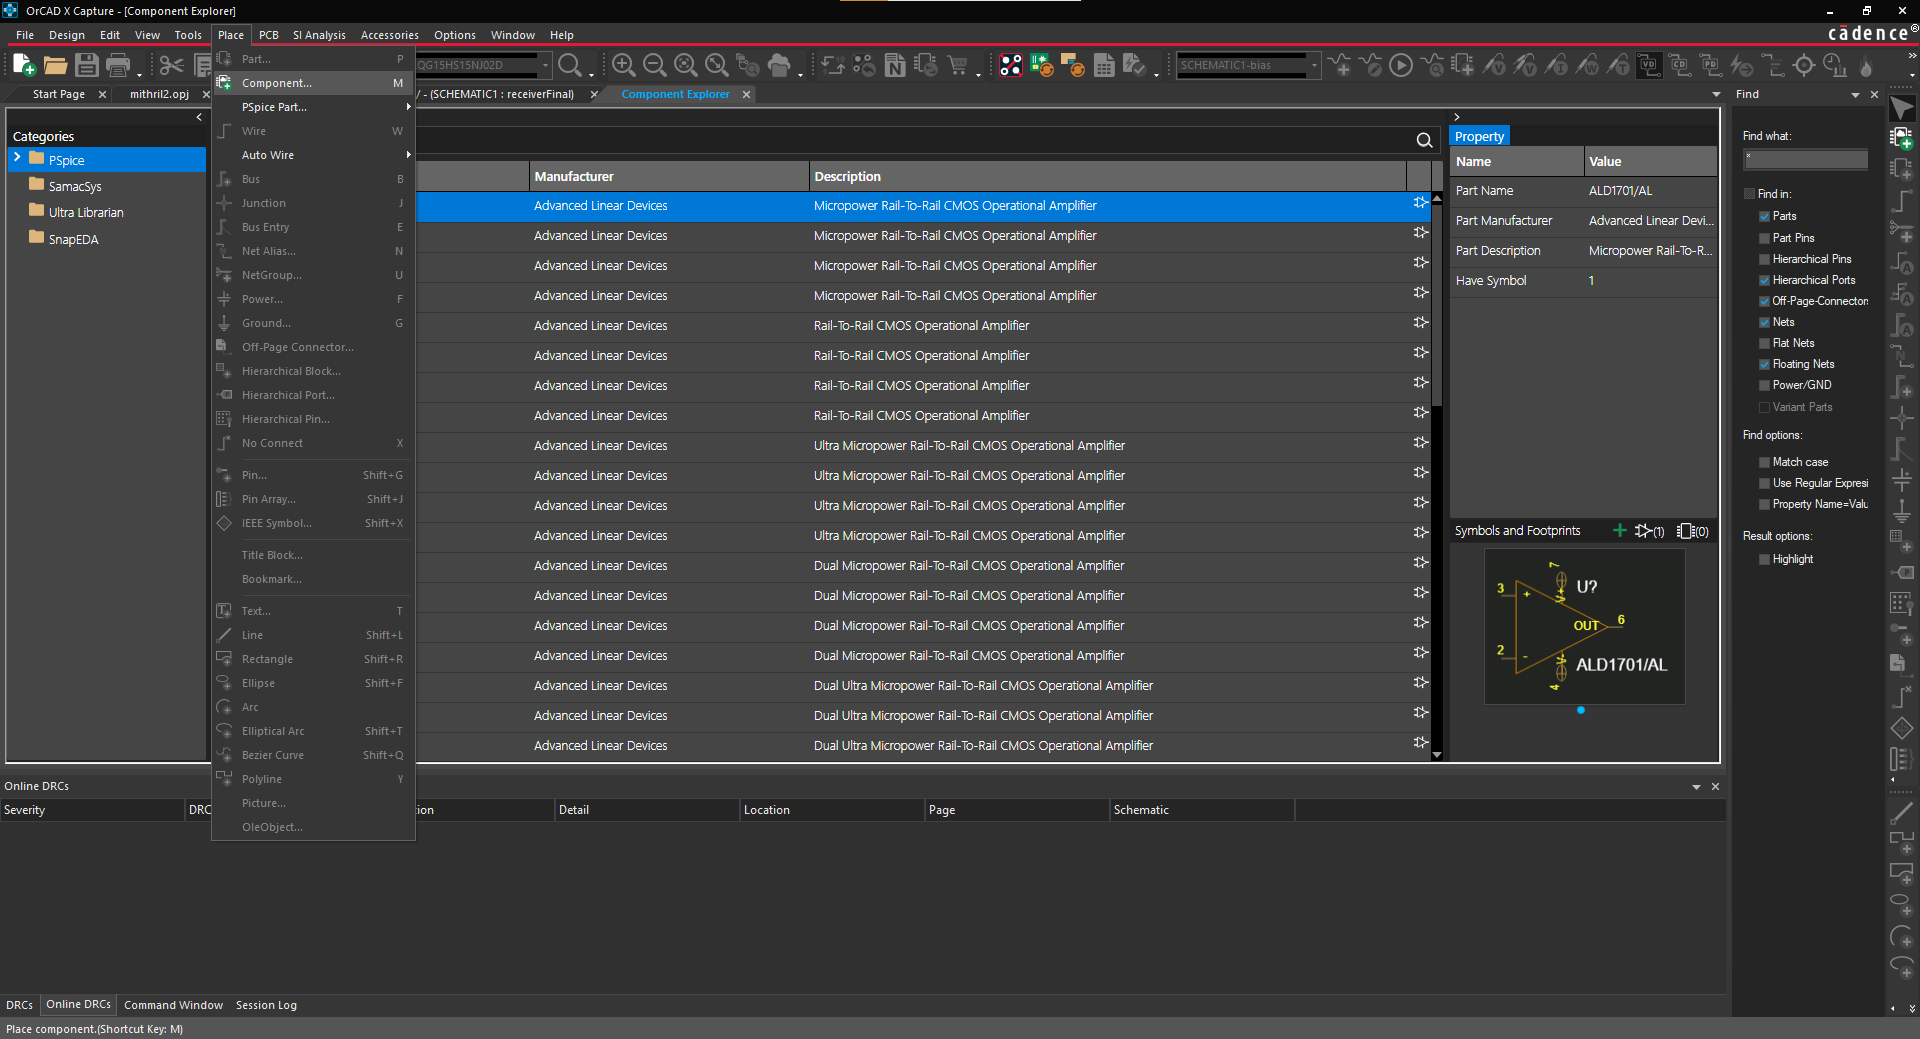
\includegraphics{CaptureImages/ultralib.png}}
\caption{Component Database Search}
\label{img:ultralib}
\end{figure}

The first important feature we found was the component database, which can be seen in Figure \ref{img:ultralib}. By clicking on the icon that has a small chip and cloud will 
take you to this page which contains subdirectories "PSpice" "SamacSys" "UltraLibrarian" and "SnapEDA". PSpice contains parts that
have simulation properties, but we ignored this as we did not know how to use PSpice. The other three are different databases
containing schematic symbols and layout footprints for parts that can be found on major retailers like DigiKey, Mouser, and Arrow.

\begin{figure}[H]
  \scalebox{.5}{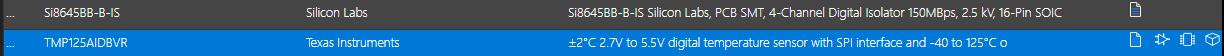
\includegraphics{CaptureImages/ultralibexample.png}}
\caption{Schematic/Footprint Examples}
\label{img:ultralibexample}
\end{figure}

You can search for parts in the search fields for the different databases to try to find a part that has a schematic symbol
and footprint available. You can see in Figure \ref{img:ultralibexample} that parts with the symbol and footprint available will
have an amp and chip symbol next to them. The box means there is a 3D CAD model associated with them too. If you cannot find
the symbol and footprint for a part, we recommend going on Mouser and finding the part, then requesting the symbol and footprint.
Usually, the schematic and footprint will be added to SamacSys after a couple of days.

\begin{figure}[H]
  \scalebox{.3}{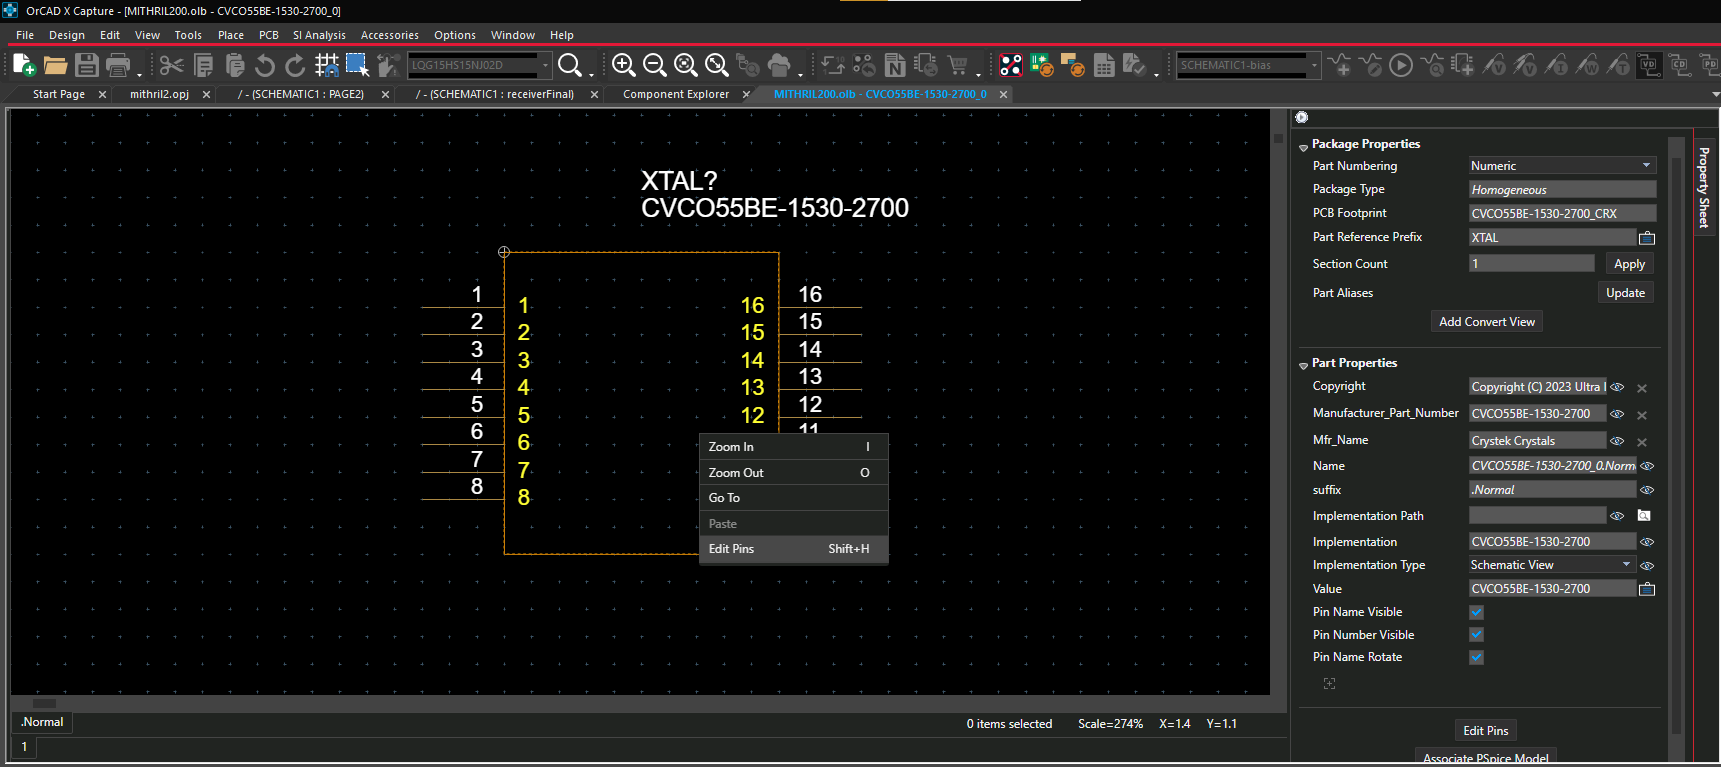
\includegraphics{CaptureImages/editpin.png}}
\caption{Editing Schematic Parts}
\label{img:editpart}
\end{figure}

Sometimes, these symbols and footprints are not correct. If the schematic symbol is incorrectly labeled, you can edit the part,
then click edit pins to make sure all the pins are correctly labeled and numbered as can be seen in Figure \ref{img:editpart}.

\begin{figure}[H]
  \scalebox{.3}{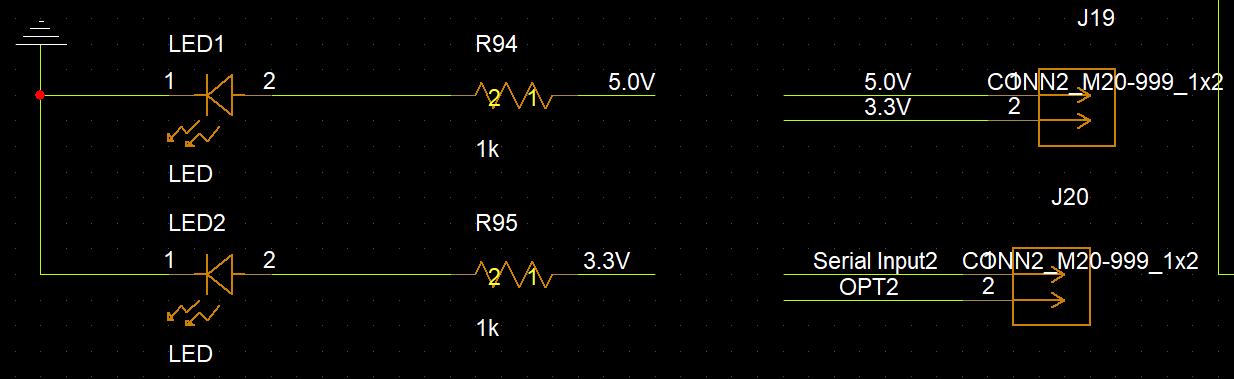
\includegraphics{CaptureImages/wirealias.png}}
\caption{Wires and Net Alias}
\label{img:wirealias}
\end{figure}

Once you've placed your parts down in the schematic, now comes time to connect everything together. To navigate through the
schematic interface, you can use CTRL+Scroll Wheel to zoom in and out, and middle mouse button to scroll left to right.

You can use "w" to enter wiring mode, which lets you place down wires according to your grid size. After wiring, be sure to use
"n" to enter net alias mode and assign aliases to your wires. As can be seen in Figure \ref{img:wirealias}, there are two
non-connected wires both with the alias "5.0V". This effectively connects them since they are under the same alias and will also
label them in the layout when routing. Using the net alias helps with things like power where connecting everything that needs
power with a wire to your power source would make the schematic a mess. In short, all wires with the same net alias are considered
connected.

\begin{figure}[H]
  \scalebox{.3}{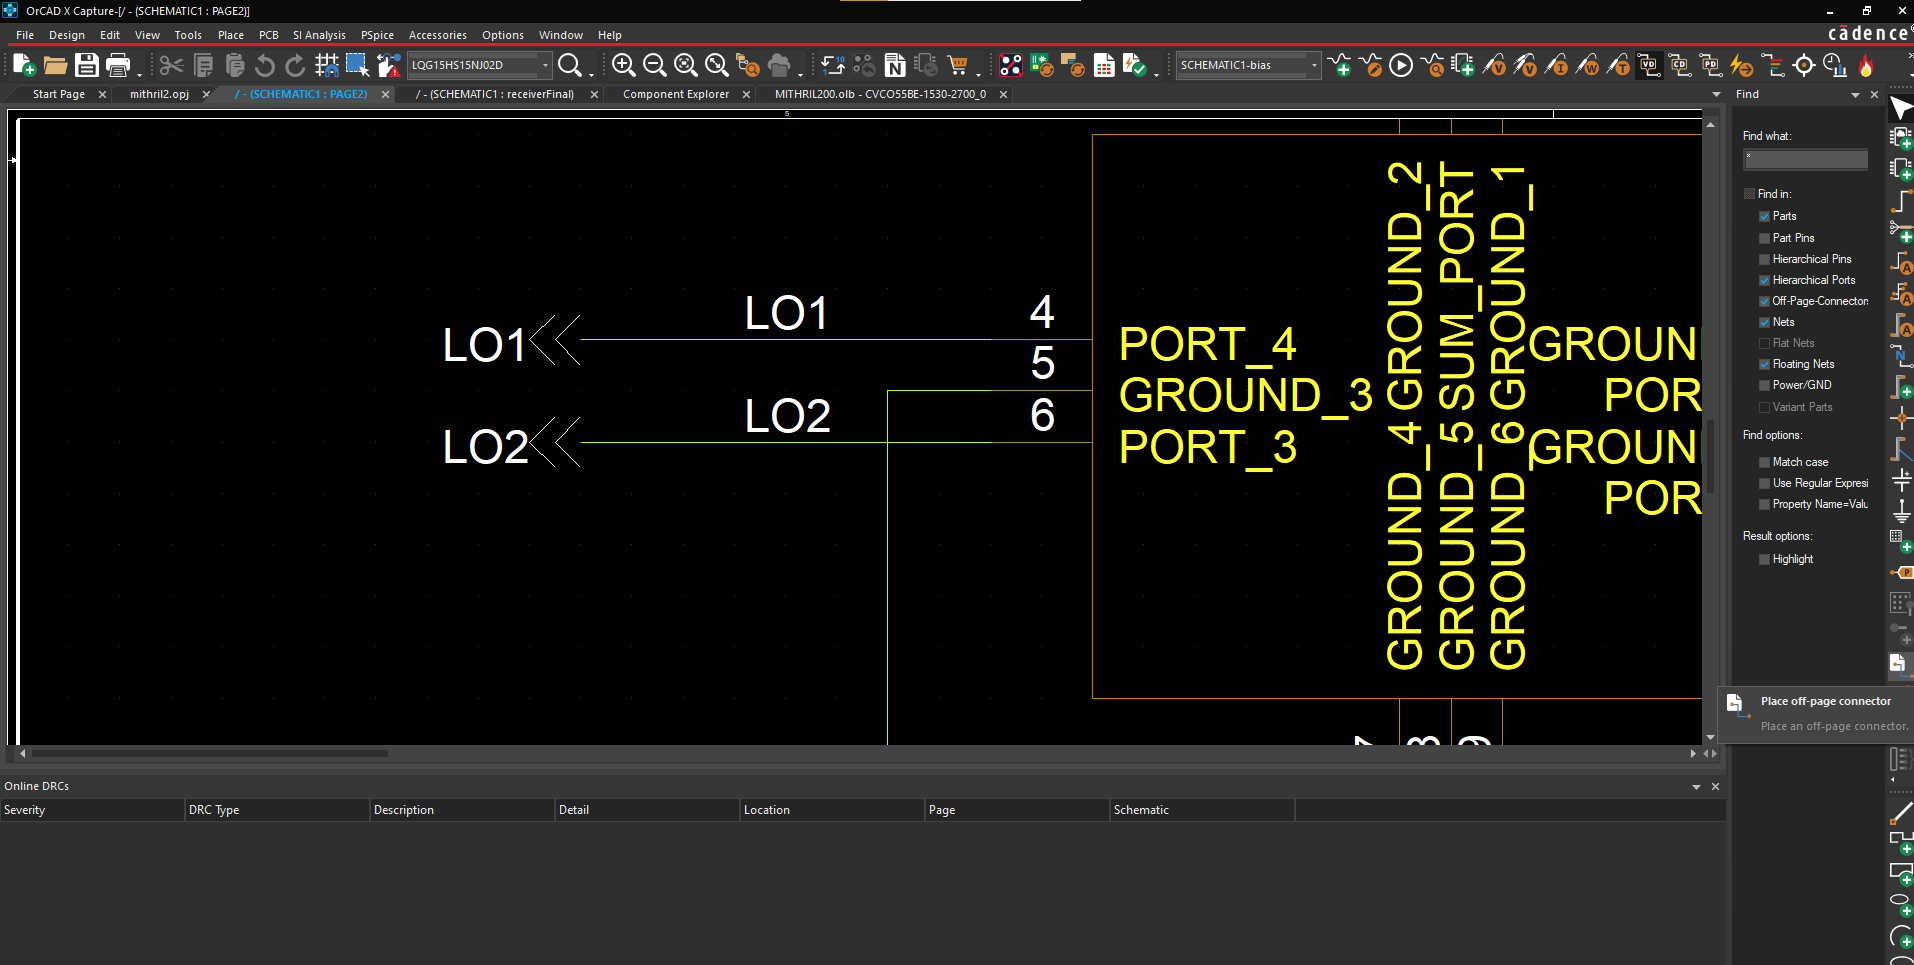
\includegraphics{CaptureImages/offpageconn.png}}
\caption{Off Page Connectors}
\label{img:offpageconn}
\end{figure}

If you run out of room or want to separate your schematics into different pages, you can connect wires from different schematic
pages using off-page connectors as shown in Figure \ref{img:offpageconn}. Connect the off-page connector to a wire and name it
the same on both schematic pages to have the wires connect.

\subsection{Circuitry Good Practices}
\subsection{Transmitter}
\subsection{Receiver}

\section{Layout}
\